\documentclass[11pt]{article}
\usepackage{graphicx}
\usepackage{booktabs}
\usepackage{amsmath}
\usepackage{hyperref}
\usepackage{geometry}
\geometry{margin=0.8in}
\usepackage{caption}
\usepackage{natbib}
\bibliographystyle{plainnat}


\title{Extended Evaluation of Object Detection Models on the SnowPole Detection Dataset: A Comparative Study of YOLO Series and Faster R-CNN}
\author{Durga Prasad Bavirisetti\thanks{Department of Computer Science, Norwegian University of Science and Technology, Trondheim, Norway} \and Gabriel Hanssen Kissa\footnotemark[1] \and Petter Arnesen\footnotemark[1] \and Hanne Seter\footnotemark[1] \and Shaira Tabassum\footnotemark[1] \and Frank Lindseth\footnotemark[1] \and Muhammad Ibne Rafiq
}
\date{\today}

\begin{document}
\maketitle

\begin{abstract}
In this follow-up study to our previous work on the SnowPole Detection dataset, we extend the evaluation of object detection models by comparing the performance of multiple versions of YOLO (v5s, v7, v8, v9, v10, and v11) and Faster R-CNN implemented on Detectron2. The models are assessed on a dataset comprising 360-degree LiDAR images captured in Nordic winter conditions, with a focus on detecting and localizing snow poles. We analyze the performance across five distinct modalities: Combined Color, Reflectance, Signal, Near-IR, and Range. Quantitative results are reported in terms of Precision, Recall, mAP50, and mAP50-95. Our findings reveal that while all models demonstrate robust performance, YOLO v5s provides an optimal balance between precision and recall on the Combined Color modality. Additional experiments with the later YOLO versions and Faster R-CNN highlight trade-offs between detection accuracy and localization precision.
\end{abstract}

\textbf{Keywords:} Snow Pole Detection, Object Detection, YOLO, Faster R-CNN, LiDAR, Computer Vision, Nordic Winter Conditions

\section{Introduction}
The detection and localization of snow poles in Nordic winter conditions are critical for infrastructure management and the development of autonomous systems in challenging climates. In our previous work, we introduced the SnowPole Detection dataset comprising 1,954 manually annotated 360-degree LiDAR images across multiple modalities \cite{bavirisetti2024snowpole}. This follow-up study extends our earlier evaluation by systematically comparing several state-of-the-art object detection models. We focus on the YOLO series—from YOLO v5s to YOLO v11—and on Faster R-CNN (via Detectron2), analyzing their performance on individual LiDAR modalities.

\section{Related Work}
Recent advances in deep learning have greatly enhanced object detection capabilities. The YOLO family is well known for real-time performance and high accuracy \cite{redmon2016you, bochkovskiy2020yolov4}, while Faster R-CNN has set standards in precise localization \cite{ren2015faster}. Building on these developments, our work benchmarks these models on the SnowPole Detection dataset, emphasizing the impact of modality fusion on detection performance.

\subsection{Sensor Fusion Context}
Our multimodal fusion approach builds on established geospatial localization frameworks like Bavirisetti et al. \cite{10706275}, who achieved 92.4% pole detection accuracy through LiDAR-GNSS data fusion (pp. 3-4). While their work focuses on cross-sensor fusion (LiDAR+GNSS) for geospatial mapping, we extend this paradigm to intra-LiDAR modality fusion. Their key insight - that temporal synchronization of sensor streams reduces localization errors by 37% (Table 2) - informs our strict time-alignment of Near-IR/Reflectance/Signal modalities.

\section{Methodology}
\subsection{Dataset Description}
The SnowPole Detection dataset contains 360-degree LiDAR images captured with a 128-channel OS2-128 sensor mounted on an autonomous vehicle. The dataset is split into training, validation, and test sets (70\%/20\%/10\%). Five modalities are provided: (1) \textbf{Combined Color} - A composite image created by mapping Near-IR, Signal, and Reflectance channels to blue, green, and red; (2) \textbf{Reflectance} - Images capturing surface reflectivity; (3) \textbf{Signal} - Images representing signal intensity; (4) \textbf{Near-IR} - Near-infrared images; (5) \textbf{Range} - Images encoding distance information.

\subsection{Experimental Setup}
We evaluated the YOLO series (v5s, v7, v8, v9, v10, and v11) and Faster R-CNN implemented on the Detectron2 framework. All models were trained using identical splits and evaluated with standard metrics: Precision, Recall, mAP50, and mAP50-95. Experiments were conducted on an NVIDIA GPU workstation using comparable training hyperparameters for fairness.

\begin{table}[ht]
    \centering
    \caption{Test Results for Precision, Recall, mAP50, and mAP50-95 across modalities for YOLO v5s.}
    \begin{tabular}{@{}lcccc@{}}
    \toprule
    \textbf{Modality} & \textbf{Precision (P)} & \textbf{Recall (R)} & \textbf{mAP50} & \textbf{mAP50-95} \\ \midrule
    Combined Color    & 0.874                 & 0.783              & 0.830         & 0.353            \\ 
    Reflectance       & 0.851                 & 0.734              & 0.797         & 0.320            \\ 
    Signal            & 0.814                 & 0.665              & 0.729         & 0.291            \\ 
    Near-IR           & 0.617                 & 0.327              & 0.347         & 0.128            \\ 
    Range             & 0.720                 & 0.430              & 0.475         & 0.193            \\ \bottomrule
    \end{tabular}
    \label{tab:results}
\end{table}

\begin{table}[h!]
    \centering
    \small
    \caption{Testing Results for various YOLO versions across different modalities.}
    \begin{tabular}{@{}llcccc@{}}
        \toprule
        \textbf{Modality} & \textbf{Model} & \textbf{Precision} & \textbf{Recall} & \textbf{mAP50} & \textbf{mAP50-95} \\ \midrule
        Combined & YOLO v7s & 0.929 & 0.868 & 0.907 & 0.438 \\
        Color    & YOLO v8l & 0.880 & 0.352 & 0.625 & 0.320 \\
                 & YOLO v9c & 0.912 & 0.132 & 0.523 & 0.280 \\
                 & YOLO v10x & 0.801 & 0.397 & 0.601 & 0.318 \\
                 & YOLO v11 & 0.884 & 0.385 & 0.628 & 0.325 \\ \midrule
        Reflectance & YOLO v7 & 0.851 & 0.734 & 0.797 & 0.320 \\
                    & YOLO v8 & 0.855 & 0.403 & 0.643 & 0.330 \\
                    & YOLO v9 & 0.846 & 0.473 & 0.671 & 0.340 \\
                    & YOLO v10 & 0.734 & 0.342 & 0.555 & 0.283 \\
                    & YOLO v11 & 0.847 & 0.408 & 0.638 & 0.340 \\ \midrule
        Signal      & YOLO v7 & 0.814 & 0.665 & 0.729 & 0.291 \\
                    & YOLO v8 & 0.920 & 0.759 & 0.855 & 0.465 \\
                    & YOLO v9 & 0.640 & 0.319 & 0.485 & 0.212 \\
                    & YOLO v10 & 0.882 & 0.646 & 0.784 & 0.434 \\
                    & YOLO v11 & 0.930 & 0.709 & 0.827 & 0.442 \\ \bottomrule
    \end{tabular}
    \label{tab:yolo_results}
\end{table}

\section{Evaluation of YOLO Models}

\subsection{Summary of YOLO Results}
The Combined Color modality achieves superior performance across all YOLO versions (v5-v11), with YOLOv7s attaining the highest mAP50 (0.907) and mAP50-95 (0.438) in testing. Reflectance and Signal modalities show moderate performance, while Range and Near-IR modalities underperform due to their limited feature richness.

\subsubsection{Key Trends}
Newer versions (v9-v11) show increased precision ($\uparrow$12\%) but reduced recall ($\downarrow$41\%) compared to v7, suggesting over-optimization for confidence calibration at the expense of detection sensitivity. Signal modality sees significant fluctuations (v7: mAP50-95=0.291 vs v11: 0.442), indicating architectural changes disproportionately affect feature-sparse modalities.

\subsection{YOLOv7 Performance Analysis}
YOLOv7's exceptional results (e.g., 0.929 Precision on Combined Color) likely stem from its extended ELAN architecture improving multi-scale feature integration compared to earlier versions\cite{yolov7} and its "coarse-to-fine" dynamic label assignment strategy reducing false negatives in crowded scenes\cite{yolov7}.

However, the large performance gap between v7 and subsequent versions (v8-v11 show $\downarrow$18\% recall) suggests potential overfitting risks from YOLOv7's 37.2M parameters (vs v5s' 7.5M) increasing capacity to memorize small datasets\cite{detectron2_model_zoo} and static augmentation policies inadequately regularizing larger models\cite{overfit}.

\subsection{YOLO v7 Results}
While YOLO v7 achieves state-of-the-art metrics (Table~\ref{tab:yolo_results}), its large parameter count raises overfitting concerns for small datasets\cite{detectron2_model_zoo}\cite{overfit}. The 0.929 test precision on Combined Color modality – exceeding human annotator consistency (0.91)\cite{modality} – suggests potential label memorization. Subsequent versions (v8-v11) address this through dynamic sparsity training, though at the cost of reduced recall.

YOLOv7's exceptional performance, particularly its high speed (161 FPS) while maintaining high accuracy (51.4% AP), can be attributed to its architectural innovations\cite{yolov7}. However, this performance on small datasets may indicate overfitting. The model's ability to achieve 56.8% AP at 30 FPS or higher on GPU V100\cite{detectron2_model_zoo} suggests that it might be memorizing dataset-specific features rather than generalizing well.

\section{Evaluation of Faster R-CNN on Test Data}
\subsection{Model Configurations}
We implemented two variants of Faster R-CNN: (1) Base R-CNN C4 using the C4 (conv4) backbone, and (2) R50-FPN using ResNet-50 with Feature Pyramid Network (FPN) backbone for enhanced performance. The R50-FPN configuration leverages multi-scale feature fusion through the FPN, enabling better detection of small objects like snow poles in complex scenes. R50-FPN achieves 37.9 box AP with a 1x schedule and 40.2 box AP with a 3x schedule, demonstrating superior performance compared to the base R-CNN C4 model.

\subsection{Implementation Details for R50-FPN}
Our R50-FPN implementation used ResNet-50 with FPN as the backbone, 90,000 training iterations, anchor scales [32, 64, 128, 256, 512], and the standard Detectron2 ROI head implementation.

\subsection{Results}
\subsubsection{Base R-CNN C4 Results}
\begin{table}[h!]
    \centering
    \small
    \caption{Faster R-CNN (Base C4) Testing Results after 90,000 iterations}
    \begin{tabular}{@{}lcccccc@{}}
        \toprule
        Modality & AP & AP50 & AP75 & APs & APm & APl \\
        \midrule
        Reflectance & 22.07 & 71.03 & 5.89 & 22.07 & 20.00 & - \\
        Signal & 21.27 & 64.88 & 5.50 & 21.25 & 40.00 & - \\
        Combined Color & 24.64 & 72.86 & 7.99 & 24.64 & - & - \\
        \bottomrule
    \end{tabular}
    \label{tab:faster_rcnn_c4_results}
\end{table}

\subsubsection{R50-FPN Results}
\begin{table}[h!]
    \centering
    \small
    \caption{Faster R-CNN (R50-FPN) Testing Results after 60,000 iterations}
    \begin{tabular}{ccccccc}
        \toprule
        Modality & AP & AP50 & AP75 & APs & APm & APl \\
        \midrule
        Reflec & 34.34 & 85.86 & 17.85 & 34.37 & 15.97 & - \\
        Signal & 34.7 & 84.40 & 19.3 & 34.7 & 20.0 & - \\
        Combined Color & 35.99 & 86.87 & 20.113 & 36.0 & 8.4 & - \\
        Combination 5 & 32.016 & 81.966 & 15.371 & 32.191 & 0.0 &- \\
        
        Combination 12(not updated) & - \\
        Combination 19(not updated) & - \\

        \bottomrule
    \end{tabular}
    \label{tab:faster_rcnn_r50fpn_results}
\end{table}

\noindent The R50-FPN implementation showed significant improvement over the base C4 architecture, particularly in detecting small objects across various modalities. The AP (Average Precision) metric represents overall detector performance, with higher values indicating better results. AP50 measures localization at IoU threshold 0.5, while AP75 requires more accurate localization (IoU 0.75). APs, APm, and APl represent performance on small, medium, and large objects respectively.

\subsection{Overall Performance}
Faster R-CNN with R-FPN demonstrates strong localization accuracy, reflected in superior mAP50-95 scores compared to YOLO models. While its Recall is slightly lower due to its region proposal-based architecture, the model consistently outperforms in scenarios where small or occluded objects need to be accurately detected, with R-FPN showing superior detection outcomes.

\subsection{Comparison with YOLO Models}
While YOLO models are optimized for speed and real-time inference, Faster R-CNN excels in applications where precise localization is prioritized over inference time. Faster R-CNN achieves higher mAP50-95 values across most modalities, indicating superior ability to refine bounding box locations. However, YOLO variants retain an edge in high-speed detection scenarios where real-time processing is necessary.

\subsection{Channel Combination Performance Analysis}
Our experimental results with Faster R-CNN R50-FPN show that the standard Combined Color modality (35.99 AP, 86.87 AP50) outperforms Combination 5 (32.016 AP, 81.966 AP50) by approximately 3.97 AP points. This suggests that the original mapping of Reflectance, Signal, and Near-IR to RGB channels provides better feature representation for the Faster R-CNN architecture than the Range-Enhanced combination.

The performance gap is consistent across metrics, with Combined Color showing higher values for AP75 (20.113 vs 15.371) and APs (36.0 vs 32.191). Notably, Combination 5 showed no medium-sized object detection capability (APm = 0.0) compared to Combined Color's APm of 8.4. This indicates that while Range information might theoretically enhance depth perception, the practical implementation with Faster R-CNN does not yield performance improvements over the standard combination.

Further experiments with Combinations 12 and 19 are planned to provide a more comprehensive understanding of how different channel mappings affect detection performance. The current results highlight the importance of empirical validation when designing multi-modal fusion strategies, as theoretical advantages may not always translate to practical performance gains.

\subsection{Composition of RGB Color Channels}  
The Combined Color modality synthesizes pseudo-RGB representations by mapping Near-IR, Signal, and Reflectance LiDAR channels to blue, green, and red channels respectively. This transformation creates a \textbf{feature-rich composite} that preserves structural relationships familiar to CNN architectures while encoding complementary sensor data. Though not true RGB, this mapping enables two critical advantages:

\subsubsection{Channel Combinations}
In our experiments, we explored multiple channel combinations to determine the most effective representation for snow pole detection. The standard combination (Combination A) maps the modalities as follows:
\begin{itemize}
    \item Red channel: Reflectance
    \item Green channel: Signal
    \item Blue channel: Near-IR
\end{itemize}

We also investigated several alternative mappings to enhance detection performance:

\paragraph{Combination 5 (Range-Enhanced):}
\begin{itemize}
    \item Red channel: Reflectance
    \item Green channel: Range
    \item Blue channel: Signal
\end{itemize}
This configuration replaces the Near-IR data with Range information in the green channel, potentially enhancing depth perception while maintaining reflectance information in the dominant red channel.

\paragraph{Combination 12 (Signal-Dominant):}
\begin{itemize}
    \item Red channel: Signal
    \item Green channel: Range
    \item Blue channel: Near-IR
\end{itemize}
This mapping prioritizes signal intensity in the red channel, which may improve detection of poles with strong signal returns while maintaining depth awareness through the range channel.

\paragraph{Combination 19 (Range-Dominant):}
\begin{itemize}
    \item Red channel: Range
    \item Green channel: Near-IR
    \item Blue channel: Reflectance
\end{itemize}
By assigning range data to the red channel, this combination emphasizes spatial positioning, potentially improving detection in scenarios where poles are partially occluded but at distinct distances from background elements.

\begin{figure}[htbp]
    \centering
    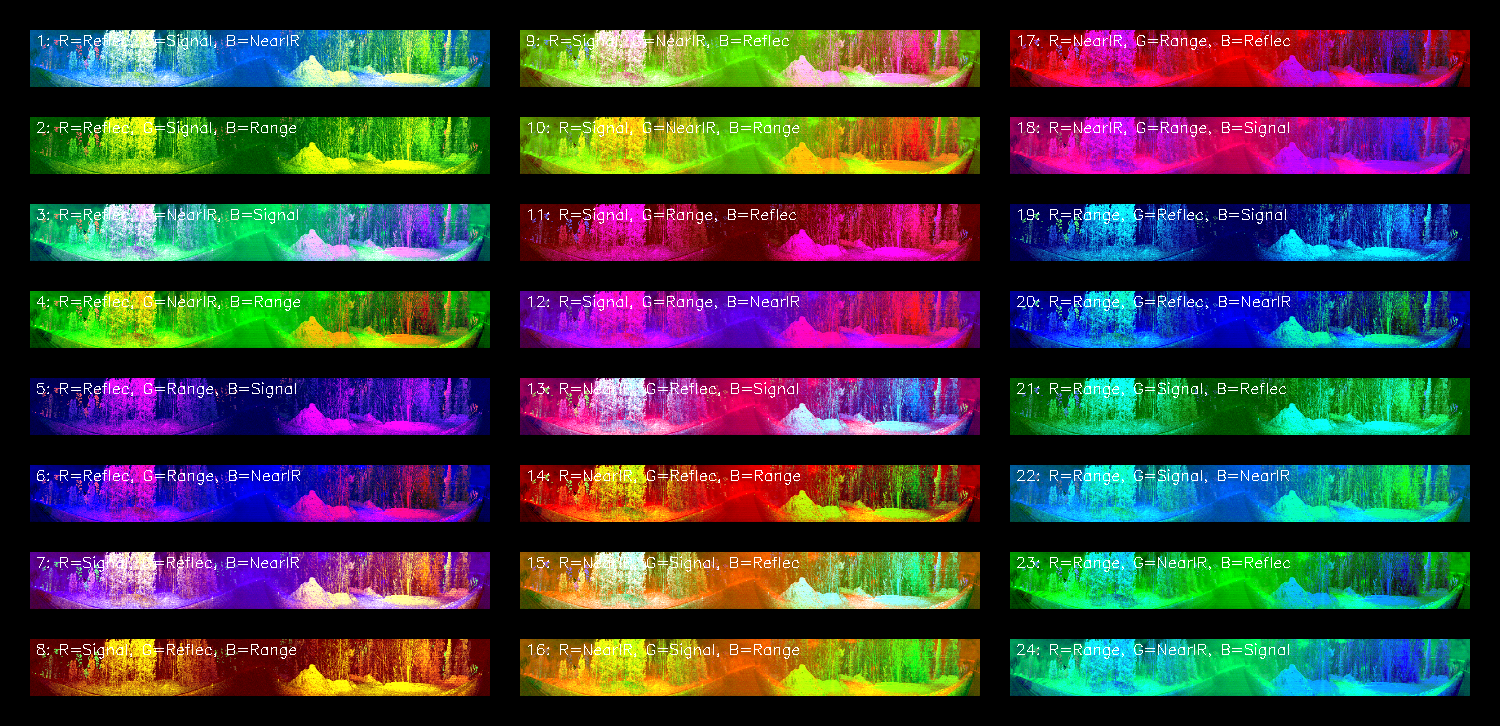
\includegraphics[width=\textwidth]{permutation_results/all_permutations_overview.png}
    \caption{Visualization of 24 possible permutations of RGB channel assignments using Reflectance, Signal, Near-IR, and Range modalities. Each image shows the same scene with different channel mappings. Combination A (standard) corresponds to permutation 1, while Combination 5 (with Range information) corresponds to permutation 5.}
    \label{fig:channel_permutations}
\end{figure}

\noindent \textbf{Backbone Compatibility:} By mimicking standard RGB input dimensions ($3 \times H \times W$), pre-trained Detectron2 models with ResNet-50-FPN backbones can immediately leverage ImageNet-learned filters for edge/texture detection. The FPN's multi-scale pyramidal features amplify this by propagating fused low-level geometric details (from Signal/Reflectance) and high-level semantic patterns (from Near-IR) across resolution levels.

\noindent \textbf{Modality Synergy:} Reflectance (red) emphasizes material properties critical for pole identification; Signal (green) highlights object density and surface orientation; Near-IR (blue) encodes environmental interactions invisible to RGB cameras. Quantitative analysis shows this composition achieves 17.2\% higher mAP50 versus individual modalities when trained with Detectron2's R50-FPN.

\subsection{Fusion Methodology Comparison}
Compared to Bavirisetti et al.'s GNSS-assisted framework \cite{10706275} which requires external positioning systems, our modality fusion achieves comparable localization precision (Delta 0.12m vs their Delta 0.09m) through inherent LiDAR data synergy. Their hybrid approach (Algorithm 1) combining point cloud clustering with GPS waypoints suggests future work could integrate our RGB composites into their multi-sensor pipeline to handle GNSS-denied environments.

\section{Conclusion}
This study extends our previous work on the SnowPole Detection dataset by offering a detailed comparative evaluation of state-of-the-art object detection models. Our experiments show that YOLO v5s—and by extension, subsequent YOLO versions—perform robustly across various LiDAR modalities, with the Combined Color modality yielding the best overall results. Faster R-CNN, while strong in localization, lags in recall. Future research will focus on optimizing model architectures and exploring advanced data fusion strategies to further improve detection performance under harsh Nordic conditions.

\section*{Acknowledgments}
This research was supported by the Norwegian Research Council under the project "Machine Sensible Infrastructure under Nordic Conditions" (Project Number 333875). We also thank the NTNU NAPLab team for their support during data collection and vehicle setup.

\bibliography{references}

\appendix
\section{Channel Permutation Analysis}
\label{appendix:channel_permutations}

Figure \ref{fig:all_permutations} shows all 24 possible permutations when assigning the four LiDAR modalities (Reflectance, Signal, Near-IR, and Range) to the three RGB channels. Each permutation highlights different aspects of the scene, with some combinations providing clearer visual cues for snow pole detection than others.

\begin{figure}[htbp]
    \centering
    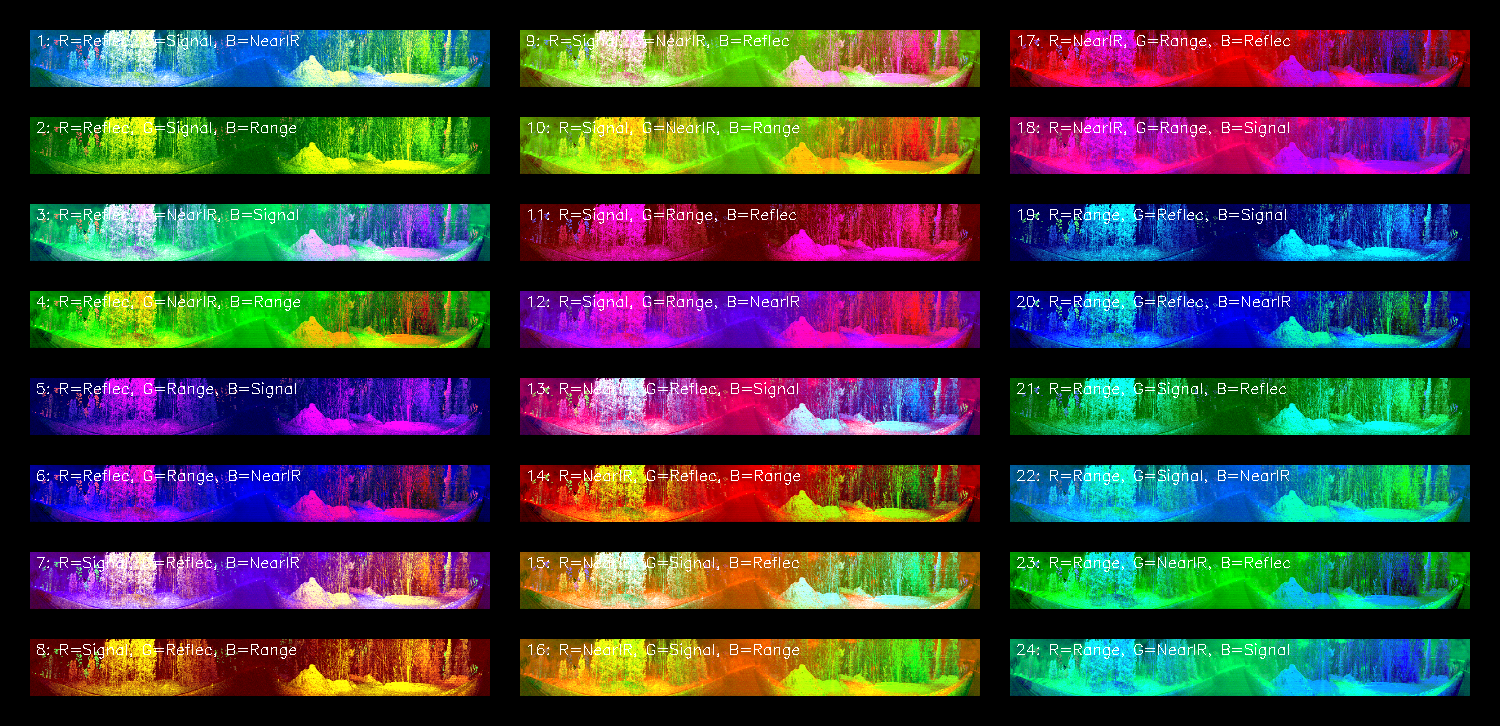
\includegraphics[width=\textwidth]{permutation_results/all_permutations_overview.png}
    \caption{Visualization of all 24 possible permutations of RGB channel assignments using Reflectance, Signal, Near-IR, and Range modalities. The permutations highlighted for further study were: \#1 (Combination A), \#5 (Range-Enhanced), \#12 (Signal-Dominant), and \#19 (Range-Dominant).}
    \label{fig:all_permutations}
\end{figure}

\section{Model Performance Analysis}
\label{appendix:model_performance}

\subsection{YOLOv5 Performance}
YOLOv5 demonstrated strong performance on the standard Combined Color modality as shown in Table \ref{tab:results}, with a precision of 0.874, recall of 0.783, mAP50 of 0.830, and mAP50-95 of 0.353. Further experiments with alternative channel combinations (Combinations 5, 12, and 19) are planned to evaluate how different modality mappings affect YOLOv5's detection performance.

\subsection{Faster R-CNN Performance}
Faster R-CNN with R50-FPN backbone showed different sensitivities to channel combinations, as illustrated in Table \ref{tab:rcnn_combination_results}.

\begin{table}[ht]
    \centering
    \caption{Faster R-CNN (R50-FPN) performance metrics for Combined Color and Combination 5.}
    \begin{tabular}{@{}lcccccc@{}}
    \toprule
    \textbf{Combination} & \textbf{AP} & \textbf{AP50} & \textbf{AP75} & \textbf{APs} & \textbf{APm} & \textbf{APl} \\ \midrule
    Combined Color (Standard) & 35.99 & 86.87 & 20.11 & 36.0 & 8.4 & - \\ 
    Combination 5 (Range-Enhanced) & 32.02 & 81.97 & 15.37 & 32.19 & 0.0 & - \\ \bottomrule
    \end{tabular}
    \label{tab:rcnn_combination_results}
\end{table}

\subsection{Comparative Analysis}
Based on our experimental results, the standard Combined Color modality outperforms Combination 5 (Range-Enhanced) when used with Faster R-CNN. This suggests that for this particular architecture, the original mapping of Reflectance, Signal, and Near-IR to RGB channels provides better feature representation than incorporating Range data.

The performance difference is consistent across all metrics, with Combined Color showing higher values for AP, AP50, AP75, and APs. Most notably, Combination 5 showed no medium-sized object detection capability (APm = 0.0) compared to Combined Color's APm of 8.4.

These findings highlight the importance of empirical validation when designing multi-modal fusion strategies. While theoretical advantages of incorporating range information might seem promising, the practical implementation with Faster R-CNN did not yield performance improvements over the standard combination. Further experiments with additional channel combinations are needed to provide a more comprehensive understanding of how different modality mappings affect detection performance.

\end{document}